\documentclass[a4paper,11pt]{article}
\usepackage{fancyhdr,graphics,graphicx,xy}
\usepackage{blkarray}
\usepackage{ifthen}
\usepackage{amssymb,amsmath,mathtools,color}
\pagestyle{fancy}
\usepackage{xparse}
\usepackage{nicematrix}
\usepackage{float}


\textwidth = 6.5 in
\textheight = 9 in
\oddsidemargin = 0.0 in
\evensidemargin = 0.0 in
\topmargin = 0.0 in
\headheight = 0.0 in
\headsep = 0.0 in
\parskip = 0.2in
\parindent = 0.0in


%%%%%%%%%%%%%%%%%%%%%%%%%%%%%%%%%%%%%%%%%%
%%% General math macros
%%%%%%%%%%%%%%%%%%%%%%%%%%%%%%%%%%%%%%%%%%


\newcommand{\asstnumber}{5}
\newcommand{\assigntop}{
  \fancyhead[L]{}
  \setlength{\headheight}{37.40004pt}
  \fancyhead[C]{\Large Math 576 -- Fall 2023\\ Assignment \asstnumber}
  \fancyhead[R]{ }
}

\newtheorem{theorem}{Theorem}
\newtheorem{corollary}[theorem]{Corollary}
\newtheorem{definition}{Definition}

\begin{document}
\assigntop

\section*{Question 3}

\subsection*{(a)}

We need to choose appropriate open subsets $U$ and $V$ of $Y$ to apply the Seifert Van-Kampen theorem. Pick a basepoint $p \in Y$ such that $p$ is inside $\Delta^2$ (a filled triangle), and let $U$ be the complement of $p$ inside $Y$. Since $p$ is a singleton $U$ is open, and let $V$, be a disc centered at $p$ such that the disc is entirely contained within the triangle surrounding $p$. Notice that $U \cap V$ is a punctured disc, which is homotopic equivalent to $S^1$, which has fundamental group $\mathbb{Z}$, thus $$ 
\pi_1 ( U \cap V) \approxeq \mathbb{Z}
$$
Since $V$ is a disc, then it has trivial fundamental group, and $U$ has a deformation retract onto the boundary of $Y$, which is just the 1-skeleton, thus 
$$
\pi(U) \simeq \{1\} \text{ and } \pi(V) \simeq G \text { for some group $G$ }
$$
\begin{figure}[H]
	\centering
	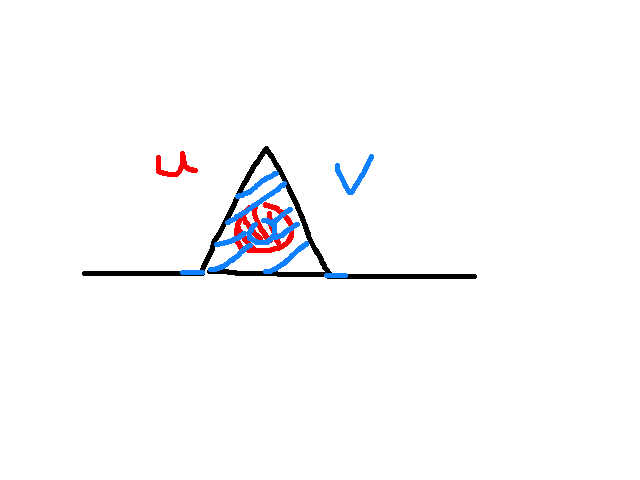
\includegraphics[width=10cm]{fig1.png}
	\caption{figure of our choices of open subsets of $Y$}
	\label{fig:1}
\end{figure}
\subsection*{(b)}


\end{document}
